\section{Thursday, February 22nd}
\subsection{Time-Frequency Duality}
Draw $\{\hat{X}_j\}\sim f_X,\quad\Xhat\in\cXhat$
\begin{shaded}
Imagine you have a set of basis functions, $\{b_j(t)\}_{j=1}^{n\to\infty}$, \\
then draw a set of coeff.'s $\{\hat{X}_j\}_{j=1}^{n\to\infty}$.\\
Set: $X(t)=\sum_{j=1}^{n}\hat{X}_j b_j(t)$.
\end{shaded}
\begin{figure}[H]
    \centering
    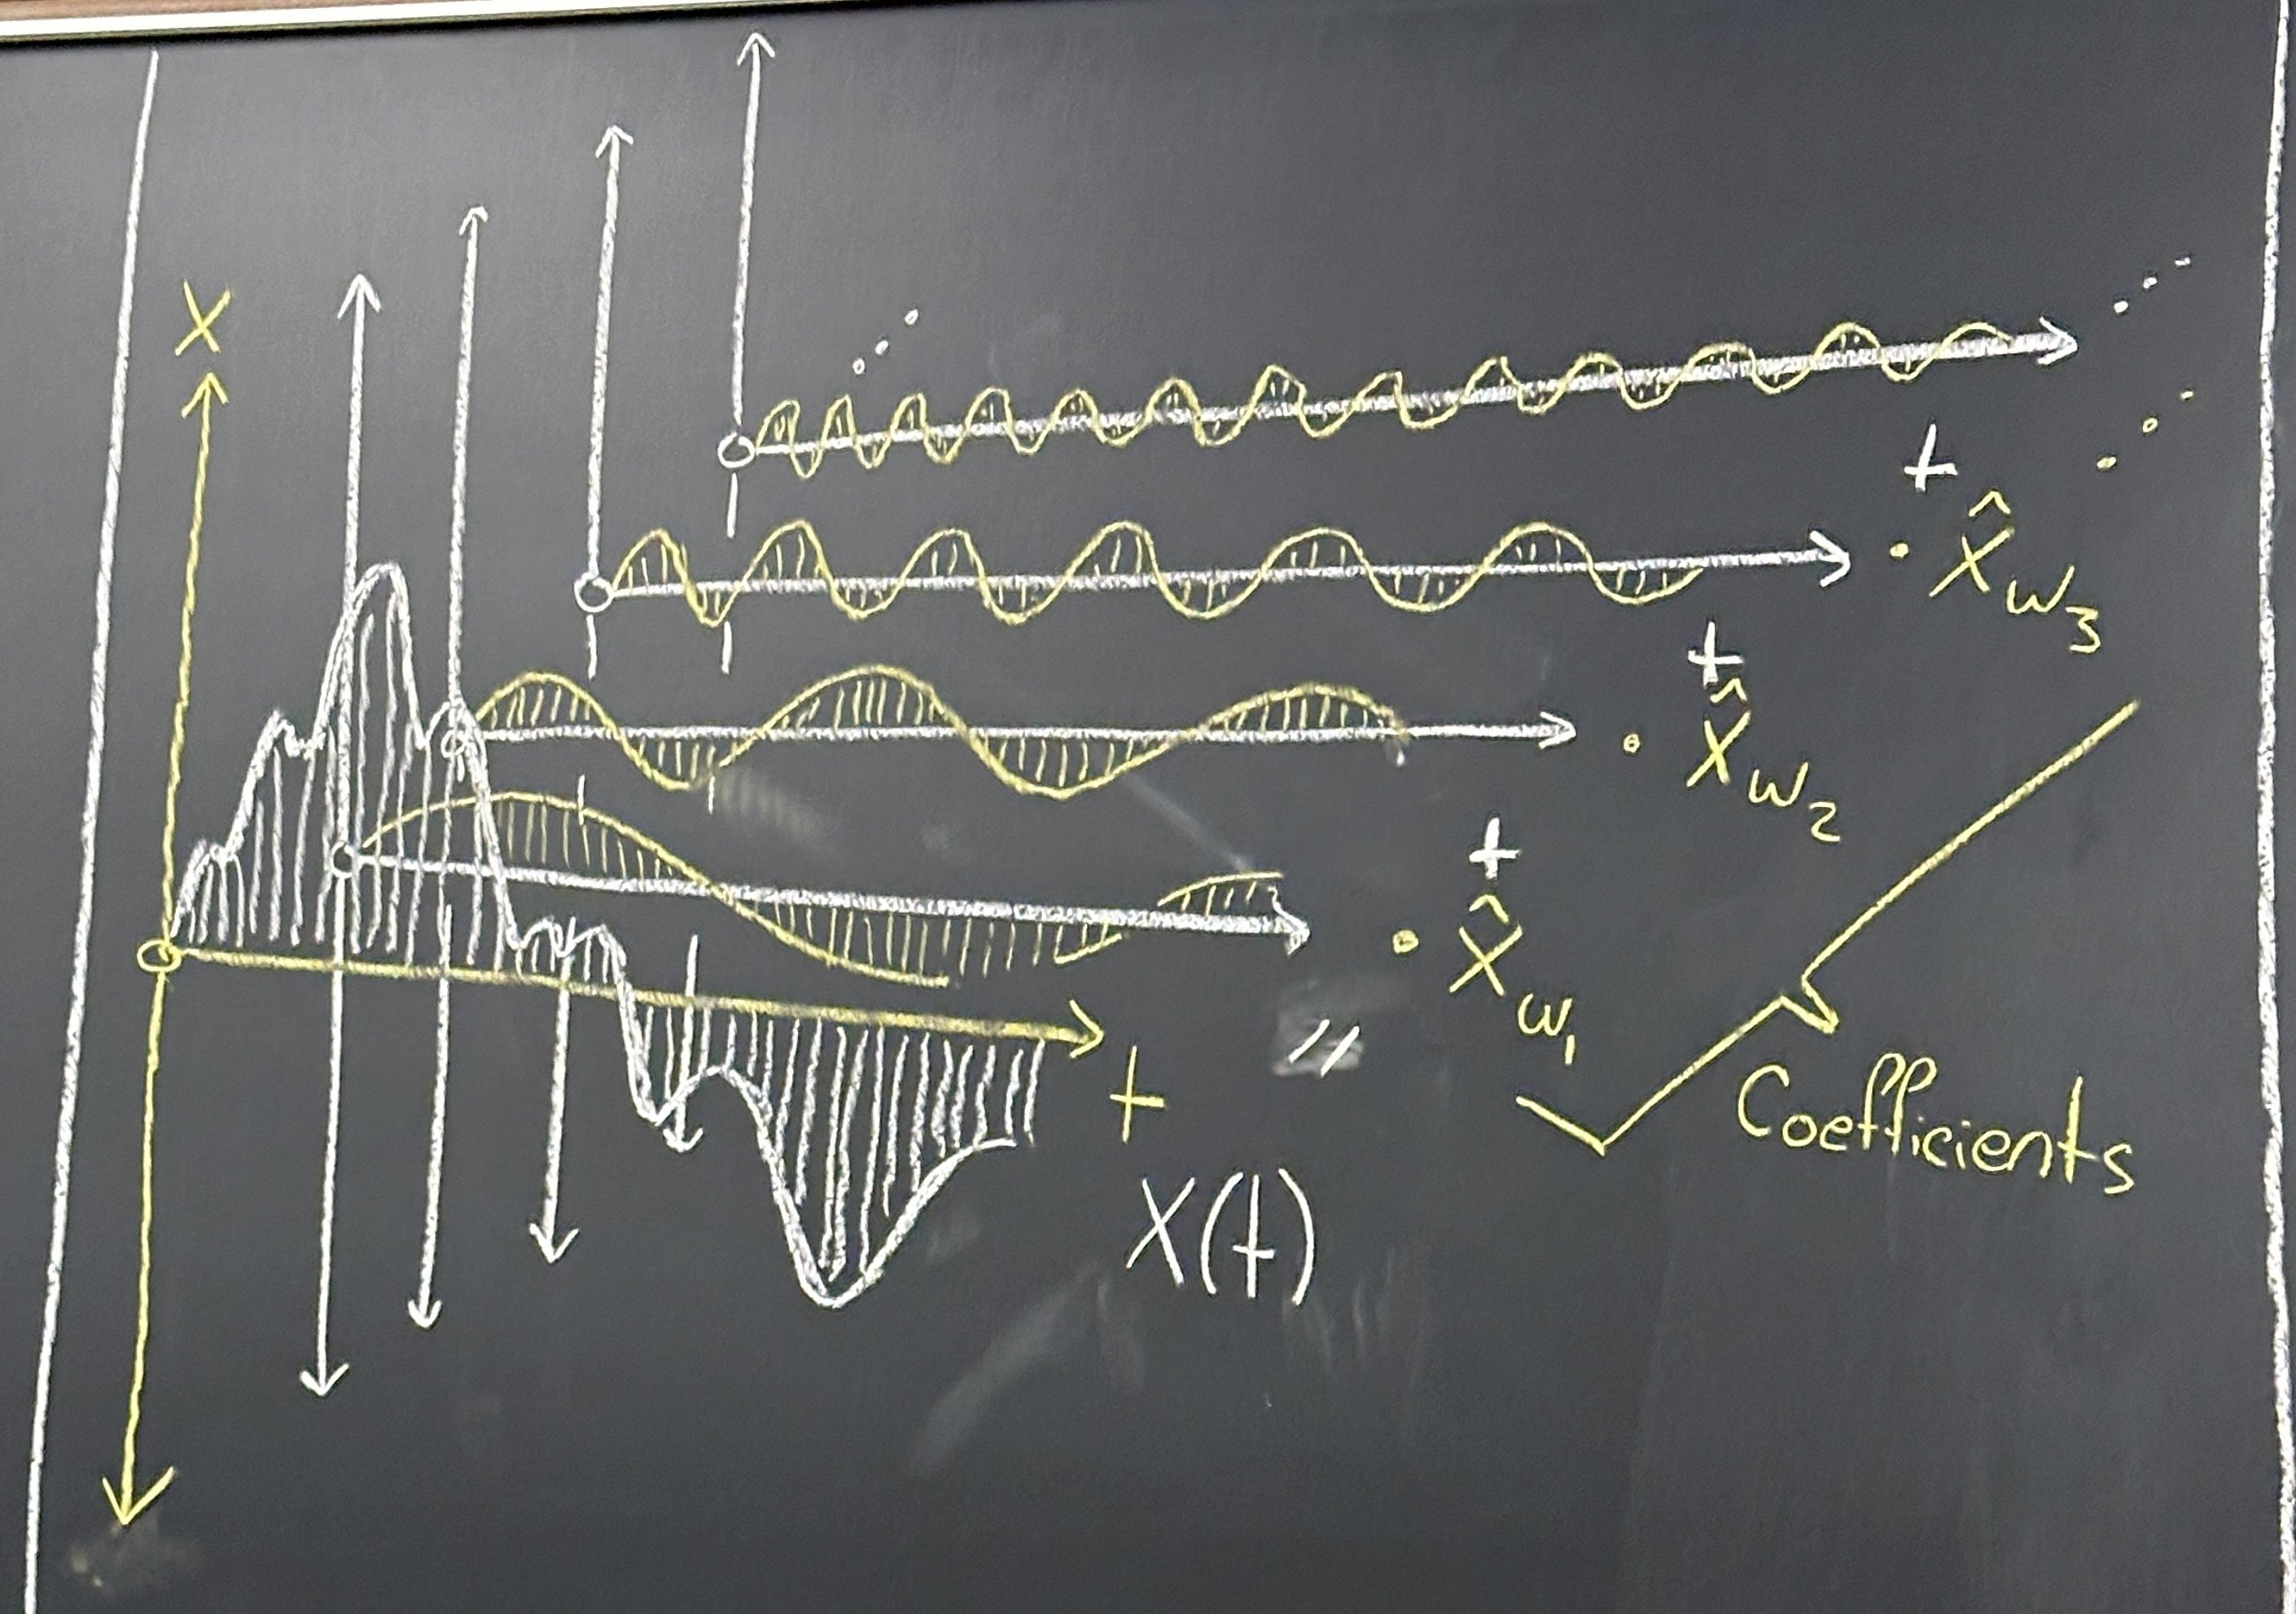
\includegraphics[scale=0.13]{lectures/wk6/img/time-freq.jpeg}
    % \caption{Caption}
    % \label{fig:enter-label}
\end{figure}

\begin{important}
Fourier transforms lose temporal resolution.
\end{important}

\subsection{Stochastic Processes}
\begin{defn}{Stochastic Process}
is a random function $X(t)$.
\end{defn}

Usually you have a SDE (\href{https://en.wikipedia.org/wiki/Stochastic_differential_equation}{Stochastic differential equation}) or a Markov process which is a random operation run conditionally fwd in time.

Here we are generating it all at once by generating a set of coeff.'s. -- this gives some curve thoroughout space.


\subsubsection{Gaussian Processes}
If we draw the set of coeff.'s to be MVG: draw $\Xhat\sim\cN$.
\begin{defn}{Gaussian Process}
$X(t)$ is a Gaussian Process if: \\
for any set of samples $\{t_j\}_{j=1}^n$\\
the r.v. $\vX=\begin{bmatrix}
    X(t_1), X(t_2), \ldots, X(t_n)
\end{bmatrix}, X_j = X(t_j)$ is drawn jointly from a MVG.
\end{defn}


It is a reasonable class of functions to be working with since it is:
\begin{enumerate}
    \item Tractable
    \item Moderately General. Note that it is not completely general, but it is one of the most simple models that gives us this level of generality.
\end{enumerate}

A MVG is uniquely specified by its mean vector 
($\mu(t)=\E[X(t)]$) 
and its covariance matrix 
$$\Sigma=K(t, s)=\Cov(X(t), X(s))=K(s, t)\st {X}\sim\cN\left(\begin{bmatrix}
 \mu(t_1) \\ \mu(t_2) \\ \vdots \\ \mu(t_n)
\end{bmatrix}, \begin{bmatrix}
 K(t_1, t_1) & K(t_2, t_2) & \cdots \\ 
 K(t_2, t_1) & K(t_2, t_2) &  \\ 
 \vdots &  & \ddots \\ 
\end{bmatrix}\right)
$$

\begin{align*}
& K(t, s)=\operatorname{Cov}[X(t), X(s)]=\sum_{j, j=1}^n E\left[\left(\hat{x}_i-\hat{\mu}_i\right)\left(\hat{x}_j-\hat{\mu}_j\right)\right] b_i(t) b_j(s)=\sum_{i j=1}^n\left[\hat{\sum}\right]_j b_i(t) b_j(s) \\
& \text { mean } \mu(t)=\mathbb{E}[X(t)] \\
& =\left[b_1(t), \ldots b_n(t)\right] \hat{\varepsilon}\begin{bmatrix}
b(s) \\
\vdots \\
b_n(s)
\end{bmatrix}=\vec{b}(t)^{\top} \hat{\dot{E}} \vec{b}(s) \\
&
\end{align*}

Suppose $\hat{x}_i \ind \hat{x}, \forall i \neq j$:\\
$
\hat{\Sigma}=\begin{bmatrix}
\hat{\sigma}_1^2 & & & \\
& \hat{\sigma}_2^2 & & \\
& & \ddots & \\
& & & \hat{\sigma}_n^2
\end{bmatrix}
$, 
then: 
$K(t, s)=\sum_{j=1}^n \hat{\sigma}^2, b_j(t) b_j(s).$

\subsection{Mercer's Theorem}
For most reasonably defined $K, \exists$ an expansion of the kind above for some, $\{b\}_{j=1}^{n \rightarrow \infty}$.

\subsection{Bochner's Theorem}
If $X(t) \sim X(t+s)$ for any $s$ then $b_j$'s are Fourier Modes.

\subsection{Shannon-Nyquist Theorem}
If $X(t)$ does not contain any frequencies higher than some band limit $B$, then $X(t)$ can be fully recovered (all the information in $X(t)$ are captured) by finitely many samples sufficiently close, $\Delta t < \frac1{2B}$.

\subsection{Entropy/Information:}
\begin{enumerate}
    \item In terms of samples, 
    \item In terms of the coeff. $\Xhat$
\end{enumerate}

$\cF\inv: 1\mapsto 2$ and $\cF: 2\mapsto 1$. Furthermore Shannon gives us this $\cF$.

\begin{shaded}
Question: How do I know that I can sample from fractional timesteps (finer samples).
\end{shaded}
This is a common question in compression, assume you are trying to store a song

Answer: Naively we could just store everything.

Well, $\vX=\begin{bmatrix}
    X(t_1), \ldots, X(t_n)
\end{bmatrix}$.\\
$\vX\sim\cN(\vmu, K)$\\
$h[\vX]=\frac12\log((2\pi e)^n |K|)=\frac12\log(|\det(K)|) +\frac{n}2\log(2\pi e)$\\
Suppose: 
\begin{flalign*}
I(\vX, \vX) &= h(\vX) - h(\vXp\mid \vX) \\
    &= h(\vX) + h(\vX) - h(\vXp, \vX)
    &&[\text{Chain Rule}]
    \\
    &= \frac12\left[\log(|K_{\Xp\Xp}|) 
    + \log(|K_{XX}|) - \log(|\begin{bmatrix}
        K_{\Xp\Xp} & K_{\Xp X}
        \\
        K_{X\Xp} K_{XX}
    \end{bmatrix}|)\right]
    \\
    &=-\frac{1}{2} \log \left(1-\rho^2\right)
\end{flalign*}


% diagram of my(t)
Smoothness of underlying GP related to MI on refined sampling.

\hrulefill

\begin{itemize}
    \item $X\sim\cN(\mu, \Sigma)$, 2D.
    \item If $\Sigma$ has SVD: $\Sigma=U \begin{bmatrix}
        \sigma_1^2 & 0 \\
        0 & \sigma_2^2 \\
    \end{bmatrix} U^\top$.
\end{itemize}
